\documentclass[1p]{elsarticle_modified}
%\bibliographystyle{elsarticle-num}

%\usepackage[colorlinks]{hyperref}
%\usepackage{abbrmath_seonhwa} %\Abb, \Ascr, \Acal ,\Abf, \Afrak
\usepackage{amsfonts}
\usepackage{amssymb}
\usepackage{amsmath}
\usepackage{amsthm}
\usepackage{scalefnt}
\usepackage{amsbsy}
\usepackage{kotex}
\usepackage{caption}
\usepackage{subfig}
\usepackage{color}
\usepackage{graphicx}
\usepackage{xcolor} %% white, black, red, green, blue, cyan, magenta, yellow
\usepackage{float}
\usepackage{setspace}
\usepackage{hyperref}

\usepackage{tikz}
\usetikzlibrary{arrows}

\usepackage{multirow}
\usepackage{array} % fixed length table
\usepackage{hhline}

%%%%%%%%%%%%%%%%%%%%%
\makeatletter
\renewcommand*\env@matrix[1][\arraystretch]{%
	\edef\arraystretch{#1}%
	\hskip -\arraycolsep
	\let\@ifnextchar\new@ifnextchar
	\array{*\c@MaxMatrixCols c}}
\makeatother %https://tex.stackexchange.com/questions/14071/how-can-i-increase-the-line-spacing-in-a-matrix
%%%%%%%%%%%%%%%

\usepackage[normalem]{ulem}

\newcommand{\msout}[1]{\ifmmode\text{\sout{\ensuremath{#1}}}\else\sout{#1}\fi}
%SOURCE: \msout is \stkout macro in https://tex.stackexchange.com/questions/20609/strikeout-in-math-mode

\newcommand{\cancel}[1]{
	\ifmmode
	{\color{red}\msout{#1}}
	\else
	{\color{red}\sout{#1}}
	\fi
}

\newcommand{\add}[1]{
	{\color{blue}\uwave{#1}}
}

\newcommand{\replace}[2]{
	\ifmmode
	{\color{red}\msout{#1}}{\color{blue}\uwave{#2}}
	\else
	{\color{red}\sout{#1}}{\color{blue}\uwave{#2}}
	\fi
}

\newcommand{\Sol}{\mathcal{S}} %segment
\newcommand{\D}{D} %diagram
\newcommand{\A}{\mathcal{A}} %arc


%%%%%%%%%%%%%%%%%%%%%%%%%%%%%5 test

\def\sl{\operatorname{\textup{SL}}(2,\Cbb)}
\def\psl{\operatorname{\textup{PSL}}(2,\Cbb)}
\def\quan{\mkern 1mu \triangleright \mkern 1mu}

\theoremstyle{definition}
\newtheorem{thm}{Theorem}[section]
\newtheorem{prop}[thm]{Proposition}
\newtheorem{lem}[thm]{Lemma}
\newtheorem{ques}[thm]{Question}
\newtheorem{cor}[thm]{Corollary}
\newtheorem{defn}[thm]{Definition}
\newtheorem{exam}[thm]{Example}
\newtheorem{rmk}[thm]{Remark}
\newtheorem{alg}[thm]{Algorithm}

\newcommand{\I}{\sqrt{-1}}
\begin{document}

%\begin{frontmatter}
%
%\title{Boundary parabolic representations of knots up to 8 crossings}
%
%%% Group authors per affiliation:
%\author{Yunhi Cho} 
%\address{Department of Mathematics, University of Seoul, Seoul, Korea}
%\ead{yhcho@uos.ac.kr}
%
%
%\author{Seonhwa Kim} %\fnref{s_kim}}
%\address{Center for Geometry and Physics, Institute for Basic Science, Pohang, 37673, Korea}
%\ead{ryeona17@ibs.re.kr}
%
%\author{Hyuk Kim}
%\address{Department of Mathematical Sciences, Seoul National University, Seoul 08826, Korea}
%\ead{hyukkim@snu.ac.kr}
%
%\author{Seokbeom Yoon}
%\address{Department of Mathematical Sciences, Seoul National University, Seoul, 08826,  Korea}
%\ead{sbyoon15@snu.ac.kr}
%
%\begin{abstract}
%We find all boundary parabolic representation of knots up to 8 crossings.
%
%\end{abstract}
%\begin{keyword}
%    \MSC[2010] 57M25 
%\end{keyword}
%
%\end{frontmatter}

%\linenumbers
%\tableofcontents
%
\newcommand\colored[1]{\textcolor{white}{\rule[-0.35ex]{0.8em}{1.4ex}}\kern-0.8em\color{red} #1}%
%\newcommand\colored[1]{\textcolor{white}{ #1}\kern-2.17ex	\textcolor{white}{ #1}\kern-1.81ex	\textcolor{white}{ #1}\kern-2.15ex\color{red}#1	}

{\Large $\underline{10_{95}~(K10a_{47})}$}

\setlength{\tabcolsep}{10pt}
\renewcommand{\arraystretch}{1.6}
\vspace{1cm}\begin{tabular}{m{100pt}>{\centering\arraybackslash}m{274pt}}
\multirow{5}{120pt}{
	\centering
	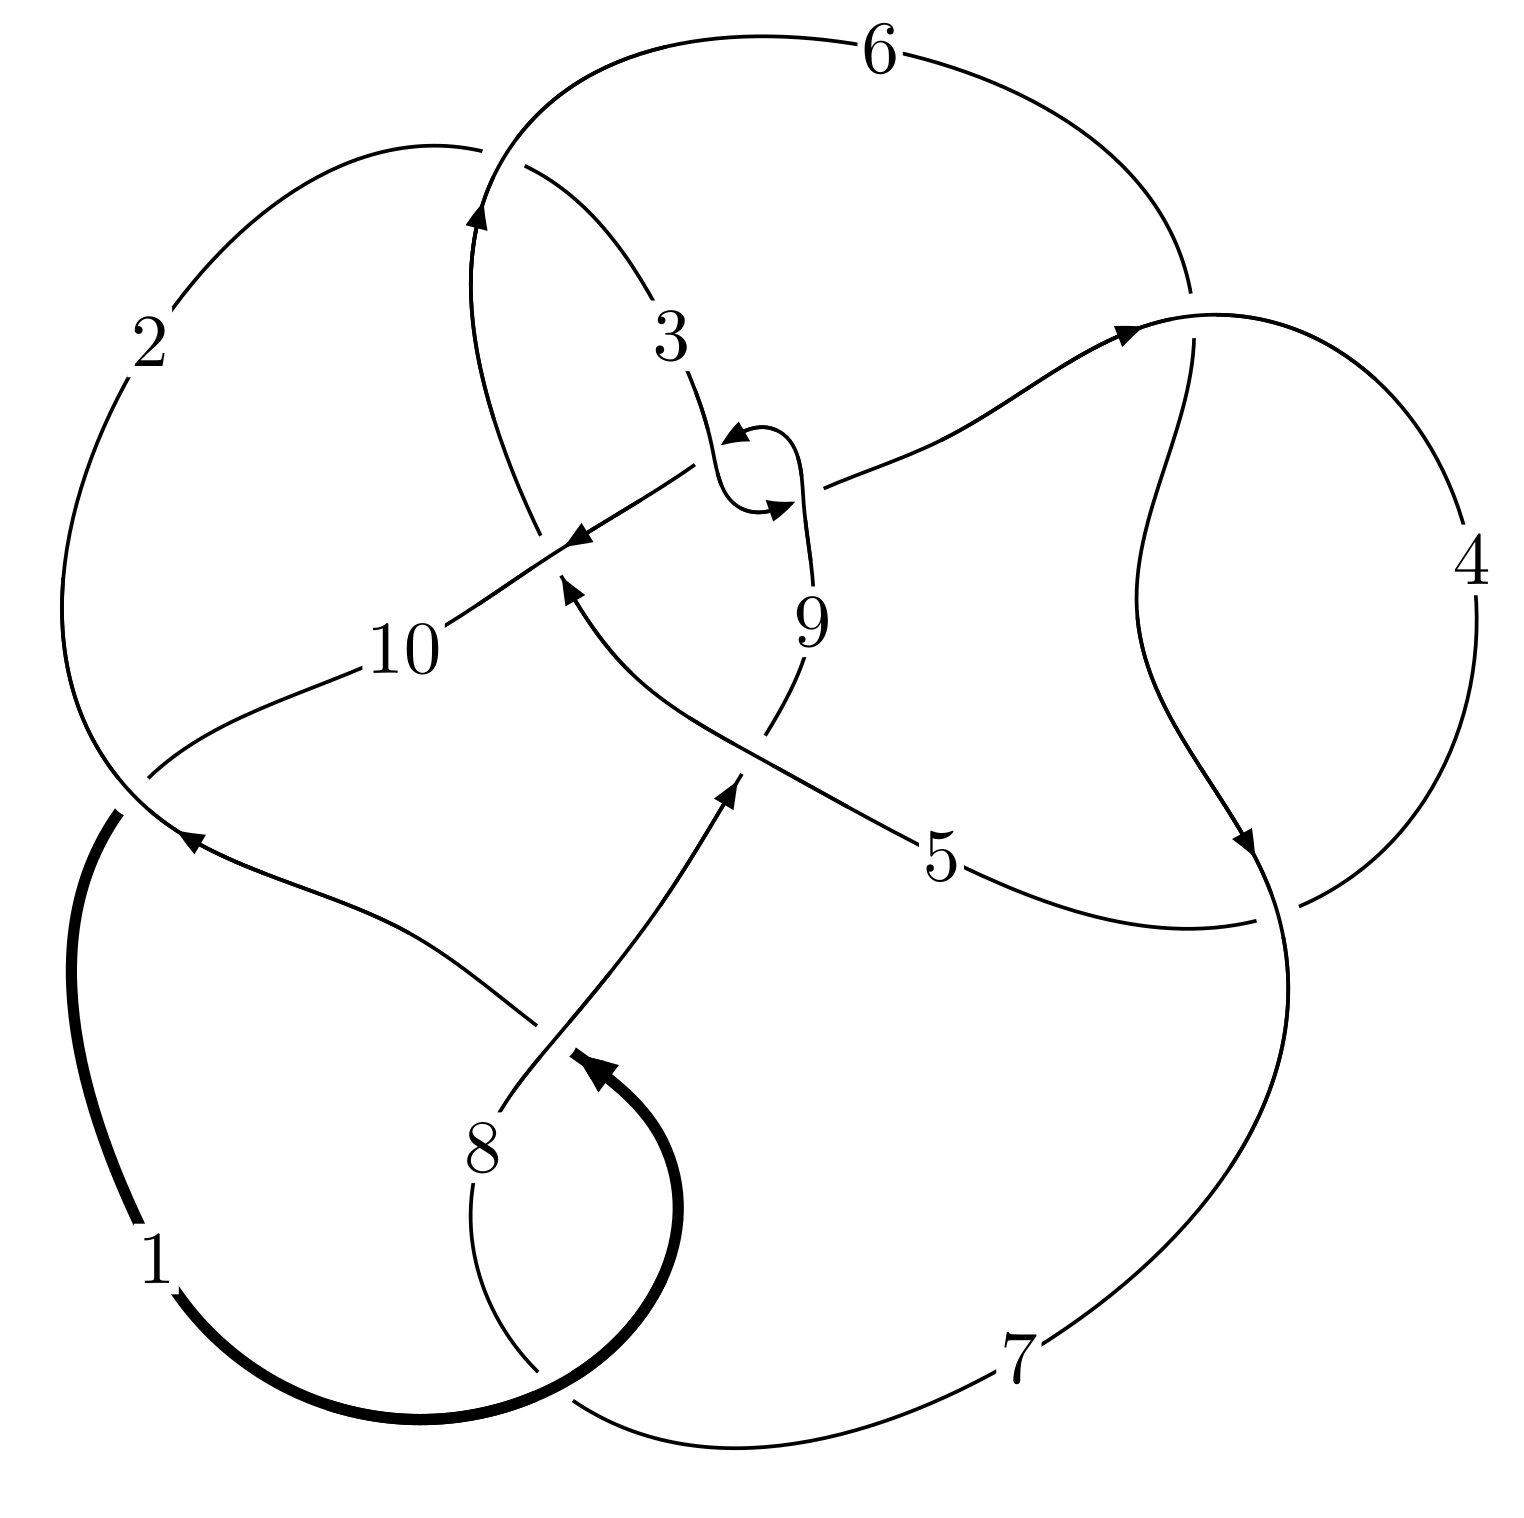
\includegraphics[width=112pt]{../../../GIT/diagram.site/Diagrams/png/179_10_95.png}\\
\ \ \ A knot diagram\footnotemark}&
\allowdisplaybreaks
\textbf{Linearized knot diagam} \\
\cline{2-2}
 &
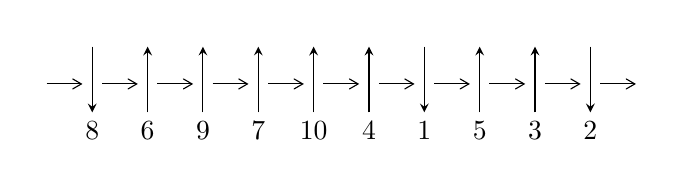
\begin{tikzpicture}[x=20pt, y=17pt]
	% nodes
	\node (C0) at (0, 0) {};
	\node (C1) at (1, 0) {};
	\node (C1U) at (1, +1) {};
	\node (C1D) at (1, -1) {8};

	\node (C2) at (2, 0) {};
	\node (C2U) at (2, +1) {};
	\node (C2D) at (2, -1) {6};

	\node (C3) at (3, 0) {};
	\node (C3U) at (3, +1) {};
	\node (C3D) at (3, -1) {9};

	\node (C4) at (4, 0) {};
	\node (C4U) at (4, +1) {};
	\node (C4D) at (4, -1) {7};

	\node (C5) at (5, 0) {};
	\node (C5U) at (5, +1) {};
	\node (C5D) at (5, -1) {10};

	\node (C6) at (6, 0) {};
	\node (C6U) at (6, +1) {};
	\node (C6D) at (6, -1) {4};

	\node (C7) at (7, 0) {};
	\node (C7U) at (7, +1) {};
	\node (C7D) at (7, -1) {1};

	\node (C8) at (8, 0) {};
	\node (C8U) at (8, +1) {};
	\node (C8D) at (8, -1) {5};

	\node (C9) at (9, 0) {};
	\node (C9U) at (9, +1) {};
	\node (C9D) at (9, -1) {3};

	\node (C10) at (10, 0) {};
	\node (C10U) at (10, +1) {};
	\node (C10D) at (10, -1) {2};
	\node (C11) at (11, 0) {};

	% arrows
	\draw[->,>={angle 60}]
	(C0) edge (C1) (C1) edge (C2) (C2) edge (C3) (C3) edge (C4) (C4) edge (C5) (C5) edge (C6) (C6) edge (C7) (C7) edge (C8) (C8) edge (C9) (C9) edge (C10) (C10) edge (C11) ;	\draw[->,>=stealth]
	(C1U) edge (C1D) (C2D) edge (C2U) (C3D) edge (C3U) (C4D) edge (C4U) (C5D) edge (C5U) (C6D) edge (C6U) (C7U) edge (C7D) (C8D) edge (C8U) (C9D) edge (C9U) (C10U) edge (C10D) ;
	\end{tikzpicture} \\
\hhline{~~} \\& 
\textbf{Solving Sequence} \\ \cline{2-2} 
 &
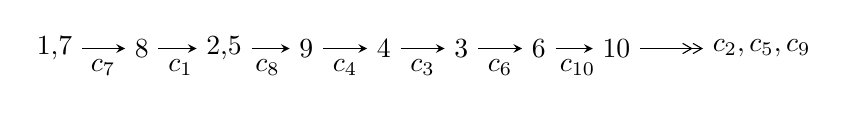
\begin{tikzpicture}[x=28pt, y=7pt]
	% node
	\node (A0) at (-1/8, 0) {1,7};
	\node (A1) at (1, 0) {8};
	\node (A2) at (33/16, 0) {2,5};
	\node (A3) at (25/8, 0) {9};
	\node (A4) at (33/8, 0) {4};
	\node (A5) at (41/8, 0) {3};
	\node (A6) at (49/8, 0) {6};
	\node (A7) at (57/8, 0) {10};
	\node (C1) at (1/2, -1) {$c_{7}$};
	\node (C2) at (3/2, -1) {$c_{1}$};
	\node (C3) at (21/8, -1) {$c_{8}$};
	\node (C4) at (29/8, -1) {$c_{4}$};
	\node (C5) at (37/8, -1) {$c_{3}$};
	\node (C6) at (45/8, -1) {$c_{6}$};
	\node (C7) at (53/8, -1) {$c_{10}$};
	\node (A8) at (9, 0) {$c_{2},c_{5},c_{9}$};

	% edge
	\draw[->,>=stealth]	
	(A0) edge (A1) (A1) edge (A2) (A2) edge (A3) (A3) edge (A4) (A4) edge (A5) (A5) edge (A6) (A6) edge (A7) ;
	\draw[->>,>={angle 60}]	
	(A7) edge (A8);
\end{tikzpicture} \\ 

\end{tabular} \\

\footnotetext{
The image of knot diagram is generated by the software ``\textbf{Draw programme}" developed by Andrew Bartholomew(\url{http://www.layer8.co.uk/maths/draw/index.htm\#Running-draw}), where we modified some parts for our purpose(\url{https://github.com/CATsTAILs/LinksPainter}).
}\phantom \\ \newline 
\centering \textbf{Ideals for irreducible components\footnotemark of $X_{\text{par}}$} 
 
\begin{align*}
I^u_{1}&=\langle 
8.96446\times10^{23} u^{44}+2.57403\times10^{24} u^{43}+\cdots+1.49180\times10^{24} b-2.95907\times10^{24},\\
\phantom{I^u_{1}}&\phantom{= \langle  }4.30182\times10^{23} u^{44}-4.12569\times10^{23} u^{43}+\cdots+1.49180\times10^{24} a-2.73959\times10^{24},\;u^{45}+3 u^{44}+\cdots+u-1\rangle \\
\\
\end{align*}
\raggedright * 1 irreducible components of $\dim_{\mathbb{C}}=0$, with total 45 representations.\\
\footnotetext{All coefficients of polynomials are rational numbers. But the coefficients are sometimes approximated in decimal forms when there is not enough margin.}
\newpage
\renewcommand{\arraystretch}{1}
\centering \section*{I. $I^u_{1}= \langle 8.96\times10^{23} u^{44}+2.57\times10^{24} u^{43}+\cdots+1.49\times10^{24} b-2.96\times10^{24},\;4.30\times10^{23} u^{44}-4.13\times10^{23} u^{43}+\cdots+1.49\times10^{24} a-2.74\times10^{24},\;u^{45}+3 u^{44}+\cdots+u-1 \rangle$}
\flushleft \textbf{(i) Arc colorings}\\
\begin{tabular}{m{7pt} m{180pt} m{7pt} m{180pt} }
\flushright $a_{1}=$&$\begin{pmatrix}0\\u\end{pmatrix}$ \\
\flushright $a_{7}=$&$\begin{pmatrix}1\\0\end{pmatrix}$ \\
\flushright $a_{8}=$&$\begin{pmatrix}1\\u^2\end{pmatrix}$ \\
\flushright $a_{2}=$&$\begin{pmatrix}- u\\- u^3+u\end{pmatrix}$ \\
\flushright $a_{5}=$&$\begin{pmatrix}-0.288363 u^{44}+0.276557 u^{43}+\cdots+0.412316 u+1.83643\\-0.600914 u^{44}-1.72545 u^{43}+\cdots-2.12140 u+1.98355\end{pmatrix}$ \\
\flushright $a_{9}=$&$\begin{pmatrix}0.0671751 u^{44}+1.09025 u^{43}+\cdots-2.21453 u-0.832290\\-0.804689 u^{44}-0.830750 u^{43}+\cdots-0.425124 u-0.467397\end{pmatrix}$ \\
\flushright $a_{4}=$&$\begin{pmatrix}0.312551 u^{44}+2.00200 u^{43}+\cdots+2.53371 u-0.147124\\-0.600914 u^{44}-1.72545 u^{43}+\cdots-2.12140 u+1.98355\end{pmatrix}$ \\
\flushright $a_{3}=$&$\begin{pmatrix}-0.288365 u^{44}-1.82727 u^{43}+\cdots+8.33577 u-2.61780\\-0.424947 u^{44}-1.44593 u^{43}+\cdots+1.13180 u+1.08626\end{pmatrix}$ \\
\flushright $a_{6}=$&$\begin{pmatrix}-0.356125 u^{44}+0.136618 u^{43}+\cdots+0.683378 u+1.78645\\-0.372015 u^{44}-1.13507 u^{43}+\cdots-1.48899 u+1.65337\end{pmatrix}$ \\
\flushright $a_{10}=$&$\begin{pmatrix}u^3\\u^5- u^3+u\end{pmatrix}$\\&\end{tabular}
\flushleft \textbf{(ii) Obstruction class $= -1$}\\~\\
\flushleft \textbf{(iii) Cusp Shapes $= \frac{1840027360774652855185796}{497267882038552304129821} u^{44}+\frac{5206472892461535459511464}{497267882038552304129821} u^{43}+\cdots+\frac{6384381127166345545265888}{497267882038552304129821} u+\frac{1812220984371614733066410}{497267882038552304129821}$}\\~\\
\newpage\renewcommand{\arraystretch}{1}
\flushleft \textbf{(iv) u-Polynomials at the component}\newline \\
\begin{tabular}{m{50pt}|m{274pt}}
Crossings & \hspace{64pt}u-Polynomials at each crossing \\
\hline $$\begin{aligned}c_{1},c_{7}\end{aligned}$$&$\begin{aligned}
&u^{45}+3 u^{44}+\cdots+u-1
\end{aligned}$\\
\hline $$\begin{aligned}c_{2}\end{aligned}$$&$\begin{aligned}
&u^{45}+5 u^{44}+\cdots-13 u-1
\end{aligned}$\\
\hline $$\begin{aligned}c_{3},c_{9}\end{aligned}$$&$\begin{aligned}
&u^{45}+3 u^{44}+\cdots+u-1
\end{aligned}$\\
\hline $$\begin{aligned}c_{4},c_{6}\end{aligned}$$&$\begin{aligned}
&u^{45}+u^{44}+\cdots+u-1
\end{aligned}$\\
\hline $$\begin{aligned}c_{5}\end{aligned}$$&$\begin{aligned}
&u^{45}+u^{44}+\cdots-11 u-1
\end{aligned}$\\
\hline $$\begin{aligned}c_{8}\end{aligned}$$&$\begin{aligned}
&u^{45}+15 u^{44}+\cdots-3 u-19
\end{aligned}$\\
\hline $$\begin{aligned}c_{10}\end{aligned}$$&$\begin{aligned}
&u^{45}+17 u^{44}+\cdots+7 u+1
\end{aligned}$\\
\hline
\end{tabular}\\~\\
\newpage\renewcommand{\arraystretch}{1}
\flushleft \textbf{(v) Riley Polynomials at the component}\newline \\
\begin{tabular}{m{50pt}|m{274pt}}
Crossings & \hspace{64pt}Riley Polynomials at each crossing \\
\hline $$\begin{aligned}c_{1},c_{7}\end{aligned}$$&$\begin{aligned}
&y^{45}-17 y^{44}+\cdots+7 y-1
\end{aligned}$\\
\hline $$\begin{aligned}c_{2}\end{aligned}$$&$\begin{aligned}
&y^{45}+107 y^{44}+\cdots+67 y-1
\end{aligned}$\\
\hline $$\begin{aligned}c_{3},c_{9}\end{aligned}$$&$\begin{aligned}
&y^{45}+27 y^{44}+\cdots+7 y-1
\end{aligned}$\\
\hline $$\begin{aligned}c_{4},c_{6}\end{aligned}$$&$\begin{aligned}
&y^{45}-29 y^{44}+\cdots+11 y-1
\end{aligned}$\\
\hline $$\begin{aligned}c_{5}\end{aligned}$$&$\begin{aligned}
&y^{45}+3 y^{44}+\cdots+35 y-1
\end{aligned}$\\
\hline $$\begin{aligned}c_{8}\end{aligned}$$&$\begin{aligned}
&y^{45}-109 y^{44}+\cdots-4893 y-361
\end{aligned}$\\
\hline $$\begin{aligned}c_{10}\end{aligned}$$&$\begin{aligned}
&y^{45}+23 y^{44}+\cdots-9 y-1
\end{aligned}$\\
\hline
\end{tabular}\\~\\
\newpage\flushleft \textbf{(vi) Complex Volumes and Cusp Shapes}
$$\begin{array}{c|c|c}  
\text{Solutions to }I^u_{1}& \I (\text{vol} + \sqrt{-1}CS) & \text{Cusp shape}\\
 \hline 
\begin{aligned}
u &= \phantom{-}0.748239 + 0.647910 I \\
a &= \phantom{-}0.403124 - 0.160622 I \\
b &= \phantom{-}1.37017 + 0.68085 I\end{aligned}
 & \phantom{-}2.77602 + 1.02408 I & \phantom{-}8.38347 - 2.46029 I \\ \hline\begin{aligned}
u &= \phantom{-}0.748239 - 0.647910 I \\
a &= \phantom{-}0.403124 + 0.160622 I \\
b &= \phantom{-}1.37017 - 0.68085 I\end{aligned}
 & \phantom{-}2.77602 - 1.02408 I & \phantom{-}8.38347 + 2.46029 I \\ \hline\begin{aligned}
u &= \phantom{-}0.890787 + 0.518116 I \\
a &= \phantom{-}1.09640 - 9.24121 I \\
b &= \phantom{-}0.973792 - 0.005327 I\end{aligned}
 & -0.05995 - 2.03640 I & \phantom{-}72.2714 - 11.7565 I \\ \hline\begin{aligned}
u &= \phantom{-}0.890787 - 0.518116 I \\
a &= \phantom{-}1.09640 + 9.24121 I \\
b &= \phantom{-}0.973792 + 0.005327 I\end{aligned}
 & -0.05995 + 2.03640 I & \phantom{-}72.2714 + 11.7565 I \\ \hline\begin{aligned}
u &= -0.820939 + 0.635302 I \\
a &= -0.253305 + 0.931796 I \\
b &= \phantom{-}1.53924 - 0.11682 I\end{aligned}
 & \phantom{-}3.59336 + 2.30367 I & \phantom{-}9.15329 - 4.83627 I \\ \hline\begin{aligned}
u &= -0.820939 - 0.635302 I \\
a &= -0.253305 - 0.931796 I \\
b &= \phantom{-}1.53924 + 0.11682 I\end{aligned}
 & \phantom{-}3.59336 - 2.30367 I & \phantom{-}9.15329 + 4.83627 I \\ \hline\begin{aligned}
u &= -0.361068 + 1.000170 I \\
a &= \phantom{-}0.351371 - 0.166844 I \\
b &= -1.073530 - 0.231341 I\end{aligned}
 & \phantom{-}1.45040 + 4.21015 I & \phantom{-}6.88936 - 10.02965 I \\ \hline\begin{aligned}
u &= -0.361068 - 1.000170 I \\
a &= \phantom{-}0.351371 + 0.166844 I \\
b &= -1.073530 + 0.231341 I\end{aligned}
 & \phantom{-}1.45040 - 4.21015 I & \phantom{-}6.88936 + 10.02965 I \\ \hline\begin{aligned}
u &= -0.557888 + 0.909903 I \\
a &= \phantom{-}0.316144 + 0.172524 I \\
b &= -1.34079 + 0.52835 I\end{aligned}
 & \phantom{-}2.54824 - 9.10382 I & \phantom{-}6.03739 + 5.00782 I \\ \hline\begin{aligned}
u &= -0.557888 - 0.909903 I \\
a &= \phantom{-}0.316144 - 0.172524 I \\
b &= -1.34079 - 0.52835 I\end{aligned}
 & \phantom{-}2.54824 + 9.10382 I & \phantom{-}6.03739 - 5.00782 I\\
 \hline 
 \end{array}$$\newpage$$\begin{array}{c|c|c}  
\text{Solutions to }I^u_{1}& \I (\text{vol} + \sqrt{-1}CS) & \text{Cusp shape}\\
 \hline 
\begin{aligned}
u &= \phantom{-}1.072010 + 0.068561 I \\
a &= \phantom{-}0.19682 + 1.79320 I \\
b &= -0.418872 + 0.891403 I\end{aligned}
 & -6.58324 + 2.11321 I & -3.96108 - 1.31750 I \\ \hline\begin{aligned}
u &= \phantom{-}1.072010 - 0.068561 I \\
a &= \phantom{-}0.19682 - 1.79320 I \\
b &= -0.418872 - 0.891403 I\end{aligned}
 & -6.58324 - 2.11321 I & -3.96108 + 1.31750 I \\ \hline\begin{aligned}
u &= -0.872155 + 0.629846 I \\
a &= -0.47083 + 1.68692 I \\
b &= \phantom{-}1.44587 + 0.31074 I\end{aligned}
 & \phantom{-}3.43558 + 2.64632 I & \phantom{-}8.92608 - 1.75211 I \\ \hline\begin{aligned}
u &= -0.872155 - 0.629846 I \\
a &= -0.47083 - 1.68692 I \\
b &= \phantom{-}1.44587 - 0.31074 I\end{aligned}
 & \phantom{-}3.43558 - 2.64632 I & \phantom{-}8.92608 + 1.75211 I \\ \hline\begin{aligned}
u &= \phantom{-}0.571052 + 0.957365 I \\
a &= \phantom{-}0.327326 - 0.019797 I \\
b &= -1.263400 - 0.274130 I\end{aligned}
 & \phantom{-}6.25575 + 2.94445 I & \phantom{-}10.14429 - 3.30426 I \\ \hline\begin{aligned}
u &= \phantom{-}0.571052 - 0.957365 I \\
a &= \phantom{-}0.327326 + 0.019797 I \\
b &= -1.263400 + 0.274130 I\end{aligned}
 & \phantom{-}6.25575 - 2.94445 I & \phantom{-}10.14429 + 3.30426 I \\ \hline\begin{aligned}
u &= -0.709910 + 0.510430 I \\
a &= \phantom{-}1.252380 - 0.161269 I \\
b &= \phantom{-}0.133311 + 0.176064 I\end{aligned}
 & -1.41864 + 2.15221 I & \phantom{-}1.64608 - 3.55734 I \\ \hline\begin{aligned}
u &= -0.709910 - 0.510430 I \\
a &= \phantom{-}1.252380 + 0.161269 I \\
b &= \phantom{-}0.133311 - 0.176064 I\end{aligned}
 & -1.41864 - 2.15221 I & \phantom{-}1.64608 + 3.55734 I \\ \hline\begin{aligned}
u &= \phantom{-}0.924885 + 0.643162 I \\
a &= -0.39182 - 2.00941 I \\
b &= \phantom{-}1.26534 - 0.87677 I\end{aligned}
 & \phantom{-}2.24019 - 6.06663 I & \phantom{-}6.70582 + 8.72697 I \\ \hline\begin{aligned}
u &= \phantom{-}0.924885 - 0.643162 I \\
a &= -0.39182 + 2.00941 I \\
b &= \phantom{-}1.26534 + 0.87677 I\end{aligned}
 & \phantom{-}2.24019 + 6.06663 I & \phantom{-}6.70582 - 8.72697 I\\
 \hline 
 \end{array}$$\newpage$$\begin{array}{c|c|c}  
\text{Solutions to }I^u_{1}& \I (\text{vol} + \sqrt{-1}CS) & \text{Cusp shape}\\
 \hline 
\begin{aligned}
u &= -0.534755 + 0.678754 I \\
a &= \phantom{-}0.767210 - 0.462986 I \\
b &= \phantom{-}0.035693 - 1.094520 I\end{aligned}
 & -1.69173 - 3.44354 I & \phantom{-}3.21684 + 3.47170 I \\ \hline\begin{aligned}
u &= -0.534755 - 0.678754 I \\
a &= \phantom{-}0.767210 + 0.462986 I \\
b &= \phantom{-}0.035693 + 1.094520 I\end{aligned}
 & -1.69173 + 3.44354 I & \phantom{-}3.21684 - 3.47170 I \\ \hline\begin{aligned}
u &= \phantom{-}0.998803 + 0.587519 I \\
a &= -0.342999 - 1.152970 I \\
b &= \phantom{-}0.166118 - 0.793978 I\end{aligned}
 & \phantom{-}0.23783 - 4.75380 I & \phantom{-}4.82148 + 5.65384 I \\ \hline\begin{aligned}
u &= \phantom{-}0.998803 - 0.587519 I \\
a &= -0.342999 + 1.152970 I \\
b &= \phantom{-}0.166118 + 0.793978 I\end{aligned}
 & \phantom{-}0.23783 + 4.75380 I & \phantom{-}4.82148 - 5.65384 I \\ \hline\begin{aligned}
u &= -1.104260 + 0.360208 I \\
a &= -0.027368 - 0.429100 I \\
b &= -0.496724 - 0.062269 I\end{aligned}
 & -1.84860 + 1.33338 I & -2.80190 - 1.06220 I \\ \hline\begin{aligned}
u &= -1.104260 - 0.360208 I \\
a &= -0.027368 + 0.429100 I \\
b &= -0.496724 + 0.062269 I\end{aligned}
 & -1.84860 - 1.33338 I & -2.80190 + 1.06220 I \\ \hline\begin{aligned}
u &= \phantom{-}0.619855 + 0.543779 I \\
a &= \phantom{-}0.786545 + 0.529917 I \\
b &= \phantom{-}0.472137 + 0.557307 I\end{aligned}
 & \phantom{-}1.389240 + 0.109846 I & \phantom{-}8.39253 - 0.28934 I \\ \hline\begin{aligned}
u &= \phantom{-}0.619855 - 0.543779 I \\
a &= \phantom{-}0.786545 - 0.529917 I \\
b &= \phantom{-}0.472137 - 0.557307 I\end{aligned}
 & \phantom{-}1.389240 - 0.109846 I & \phantom{-}8.39253 + 0.28934 I \\ \hline\begin{aligned}
u &= -1.030460 + 0.624781 I \\
a &= -1.00464 + 1.07941 I \\
b &= -0.116882 + 1.280150 I\end{aligned}
 & -3.11090 + 8.51494 I & \phantom{-}1.12145 - 8.02650 I \\ \hline\begin{aligned}
u &= -1.030460 - 0.624781 I \\
a &= -1.00464 - 1.07941 I \\
b &= -0.116882 - 1.280150 I\end{aligned}
 & -3.11090 - 8.51494 I & \phantom{-}1.12145 + 8.02650 I\\
 \hline 
 \end{array}$$\newpage$$\begin{array}{c|c|c}  
\text{Solutions to }I^u_{1}& \I (\text{vol} + \sqrt{-1}CS) & \text{Cusp shape}\\
 \hline 
\begin{aligned}
u &= -1.158790 + 0.358173 I \\
a &= -0.174096 - 0.464304 I \\
b &= -0.614061 - 0.062005 I\end{aligned}
 & -1.84651 + 1.33386 I & -3.76295 - 1.40019 I \\ \hline\begin{aligned}
u &= -1.158790 - 0.358173 I \\
a &= -0.174096 + 0.464304 I \\
b &= -0.614061 + 0.062005 I\end{aligned}
 & -1.84651 - 1.33386 I & -3.76295 + 1.40019 I \\ \hline\begin{aligned}
u &= \phantom{-}1.230990 + 0.092992 I \\
a &= -0.98270 + 1.11992 I \\
b &= -1.097490 + 0.546794 I\end{aligned}
 & -4.42636 - 7.34032 I & \phantom{-0.000000 -}0. + 6.70183 I \\ \hline\begin{aligned}
u &= \phantom{-}1.230990 - 0.092992 I \\
a &= -0.98270 - 1.11992 I \\
b &= -1.097490 - 0.546794 I\end{aligned}
 & -4.42636 + 7.34032 I & \phantom{-0.000000 } 0. - 6.70183 I \\ \hline\begin{aligned}
u &= -0.734453 + 0.170610 I \\
a &= \phantom{-}2.20693 + 0.55929 I \\
b &= \phantom{-}0.600244 + 0.443962 I\end{aligned}
 & -1.43818 + 2.33862 I & \phantom{-}0.15315 - 3.89068 I \\ \hline\begin{aligned}
u &= -0.734453 - 0.170610 I \\
a &= \phantom{-}2.20693 - 0.55929 I \\
b &= \phantom{-}0.600244 - 0.443962 I\end{aligned}
 & -1.43818 - 2.33862 I & \phantom{-}0.15315 + 3.89068 I \\ \hline\begin{aligned}
u &= -1.099700 + 0.703989 I \\
a &= \phantom{-}0.29033 - 1.93516 I \\
b &= -1.36790 - 0.61478 I\end{aligned}
 & \phantom{-}0.8834 + 15.0479 I & \phantom{-0.000000 } 0. - 8.99569 I \\ \hline\begin{aligned}
u &= -1.099700 - 0.703989 I \\
a &= \phantom{-}0.29033 + 1.93516 I \\
b &= -1.36790 + 0.61478 I\end{aligned}
 & \phantom{-}0.8834 - 15.0479 I & \phantom{-0.000000 -}0. + 8.99569 I \\ \hline\begin{aligned}
u &= \phantom{-}1.106830 + 0.724523 I \\
a &= \phantom{-}0.16343 + 1.57481 I \\
b &= -1.291930 + 0.408785 I\end{aligned}
 & \phantom{-}4.59210 - 9.07926 I & \phantom{-0.000000 } 0 \\ \hline\begin{aligned}
u &= \phantom{-}1.106830 - 0.724523 I \\
a &= \phantom{-}0.16343 - 1.57481 I \\
b &= -1.291930 - 0.408785 I\end{aligned}
 & \phantom{-}4.59210 + 9.07926 I & \phantom{-0.000000 } 0\\
 \hline 
 \end{array}$$\newpage$$\begin{array}{c|c|c}  
\text{Solutions to }I^u_{1}& \I (\text{vol} + \sqrt{-1}CS) & \text{Cusp shape}\\
 \hline 
\begin{aligned}
u &= -1.031500 + 0.835190 I \\
a &= \phantom{-}0.505754 - 0.770326 I \\
b &= -0.907193 - 0.175723 I\end{aligned}
 & -1.04837 + 3.34425 I & \phantom{-0.000000 } 0. - 10.76892 I \\ \hline\begin{aligned}
u &= -1.031500 - 0.835190 I \\
a &= \phantom{-}0.505754 + 0.770326 I \\
b &= -0.907193 + 0.175723 I\end{aligned}
 & -1.04837 - 3.34425 I & \phantom{-0.000000 -}0. + 10.76892 I \\ \hline\begin{aligned}
u &= \phantom{-}0.406402\phantom{ +0.000000I} \\
a &= \phantom{-}1.83709\phantom{ +0.000000I} \\
b &= \phantom{-}0.702503\phantom{ +0.000000I}\end{aligned}
 & \phantom{-}1.02583\phantom{ +0.000000I} & \phantom{-}10.4140\phantom{ +0.000000I} \\ \hline\begin{aligned}
u &= \phantom{-}0.149228 + 0.309881 I \\
a &= \phantom{-}2.06545 - 0.10916 I \\
b &= \phantom{-}1.135600 - 0.215122 I\end{aligned}
 & \phantom{-}0.959713 - 1.013710 I & \phantom{-}4.02329 - 0.70963 I \\ \hline\begin{aligned}
u &= \phantom{-}0.149228 - 0.309881 I \\
a &= \phantom{-}2.06545 + 0.10916 I \\
b &= \phantom{-}1.135600 + 0.215122 I\end{aligned}
 & \phantom{-}0.959713 + 1.013710 I & \phantom{-}4.02329 + 0.70963 I\\
 \hline 
 \end{array}$$\newpage
\newpage\renewcommand{\arraystretch}{1}
\centering \section*{ II. u-Polynomials}
\begin{tabular}{m{50pt}|m{274pt}}
Crossings & \hspace{64pt}u-Polynomials at each crossing \\
\hline $$\begin{aligned}c_{1},c_{7}\end{aligned}$$&$\begin{aligned}
&u^{45}+3 u^{44}+\cdots+u-1
\end{aligned}$\\
\hline $$\begin{aligned}c_{2}\end{aligned}$$&$\begin{aligned}
&u^{45}+5 u^{44}+\cdots-13 u-1
\end{aligned}$\\
\hline $$\begin{aligned}c_{3},c_{9}\end{aligned}$$&$\begin{aligned}
&u^{45}+3 u^{44}+\cdots+u-1
\end{aligned}$\\
\hline $$\begin{aligned}c_{4},c_{6}\end{aligned}$$&$\begin{aligned}
&u^{45}+u^{44}+\cdots+u-1
\end{aligned}$\\
\hline $$\begin{aligned}c_{5}\end{aligned}$$&$\begin{aligned}
&u^{45}+u^{44}+\cdots-11 u-1
\end{aligned}$\\
\hline $$\begin{aligned}c_{8}\end{aligned}$$&$\begin{aligned}
&u^{45}+15 u^{44}+\cdots-3 u-19
\end{aligned}$\\
\hline $$\begin{aligned}c_{10}\end{aligned}$$&$\begin{aligned}
&u^{45}+17 u^{44}+\cdots+7 u+1
\end{aligned}$\\
\hline
\end{tabular}\newpage\renewcommand{\arraystretch}{1}
\centering \section*{ III. Riley Polynomials}
\begin{tabular}{m{50pt}|m{274pt}}
Crossings & \hspace{64pt}Riley Polynomials at each crossing \\
\hline $$\begin{aligned}c_{1},c_{7}\end{aligned}$$&$\begin{aligned}
&y^{45}-17 y^{44}+\cdots+7 y-1
\end{aligned}$\\
\hline $$\begin{aligned}c_{2}\end{aligned}$$&$\begin{aligned}
&y^{45}+107 y^{44}+\cdots+67 y-1
\end{aligned}$\\
\hline $$\begin{aligned}c_{3},c_{9}\end{aligned}$$&$\begin{aligned}
&y^{45}+27 y^{44}+\cdots+7 y-1
\end{aligned}$\\
\hline $$\begin{aligned}c_{4},c_{6}\end{aligned}$$&$\begin{aligned}
&y^{45}-29 y^{44}+\cdots+11 y-1
\end{aligned}$\\
\hline $$\begin{aligned}c_{5}\end{aligned}$$&$\begin{aligned}
&y^{45}+3 y^{44}+\cdots+35 y-1
\end{aligned}$\\
\hline $$\begin{aligned}c_{8}\end{aligned}$$&$\begin{aligned}
&y^{45}-109 y^{44}+\cdots-4893 y-361
\end{aligned}$\\
\hline $$\begin{aligned}c_{10}\end{aligned}$$&$\begin{aligned}
&y^{45}+23 y^{44}+\cdots-9 y-1
\end{aligned}$\\
\hline
\end{tabular}
\vskip 2pc
\end{document}